\documentclass[11pt]{article}
\usepackage[a4paper,margin=2.3cm]{geometry}
\usepackage{amsmath,amssymb,amsthm,graphicx,hyperref,xcolor}
\hypersetup{colorlinks,linkcolor=blue!50!black,urlcolor=blue!50!black,citecolor=blue!50!black}
\newtheorem{theorem}{Theorem}\newtheorem{proposition}[theorem]{Proposition}
\newtheorem{corollary}[theorem]{Corollary}
\theoremstyle{definition}\newtheorem{definition}[theorem]{Definition}\newtheorem{remark}[theorem]{Remark}
\newcommand{\C}{\mathbb{C}}\newcommand{\Z}{\mathbb{Z}}\newcommand{\R}{\mathbb{R}}\renewcommand{\Re}{\operatorname{Re}}\renewcommand{\Im}{\operatorname{Im}}
\title{Where the hidden intersections live:\\ phantom loci of plane curves in $\C^2$}
\author{Carlo Perassi}
\date{October 2026 \\ \small Technical note accompanying a reply to Inigo Quilez's YouTube Short}
\begin{document}\maketitle
\begin{abstract}
A line that misses a circle still meets it at two complex points. Inigo Quilez's Short shows this by plotting real and imaginary parts as the line wanders, and concludes that ``there are always intersections, they are just hidden.'' We make ``hidden'' precise. If the line is translated \emph{parallel to itself} instead of moved freely, the hidden points sweep a well-defined real curve inside the complexified curve, the \emph{phantom locus}. For the circle it is a hyperbola glued to the circle at the two tangency points. We prove that phantom branches leave the real curve only at tangencies, at right angles and with matching curvature. We then describe the operator $R_\lambda:(c,t)\mapsto(c,\lambda t)$ that relates a curve to its phantom, compute the stabilizer of a curve under it, and characterize the curves that are their own phantom.
\end{abstract}

\section{Introduction}
In the YouTube Short \emph{``Intersections are always there''} by Inigo Quilez (\url{https://www.youtube.com/shorts/cc-Z_igk4Lo}), a ray $p=o+\tau d$ ($|d|=1$) is intersected with a circle $|p|=r$:
\[
 p \;=\; o - d\Big(o\cdot d \pm \sqrt{(o\cdot d)^2-|o|^2+r^2}\Big).
\]
When the radicand $\Delta$ is negative, the root is replaced by $\pm i\sqrt{|\Delta|}$. The real part $o-d(o\cdot d)$ is the foot of the perpendicular from the center (blue dot). The imaginary part $\pm d\sqrt{|\Delta|}$ is drawn along the line (orange dots). As the line rotates and translates freely, the dots leave tangled trails (Fig.~\ref{fig:quilez}, left).

The tangle comes from mixing two motions. Fix the direction, translate only, and the orange trail becomes a hyperbola (Fig.~\ref{fig:quilez}, right). The 2D picture is a projection of a 3D one, in which that hyperbola stands perpendicular to the circle along an imaginary axis (Fig.~\ref{fig:locus}). This note works out the general version for any real algebraic curve. All numerical claims below were checked in Python (script \texttt{verify.py}).

\begin{figure}[t]\centering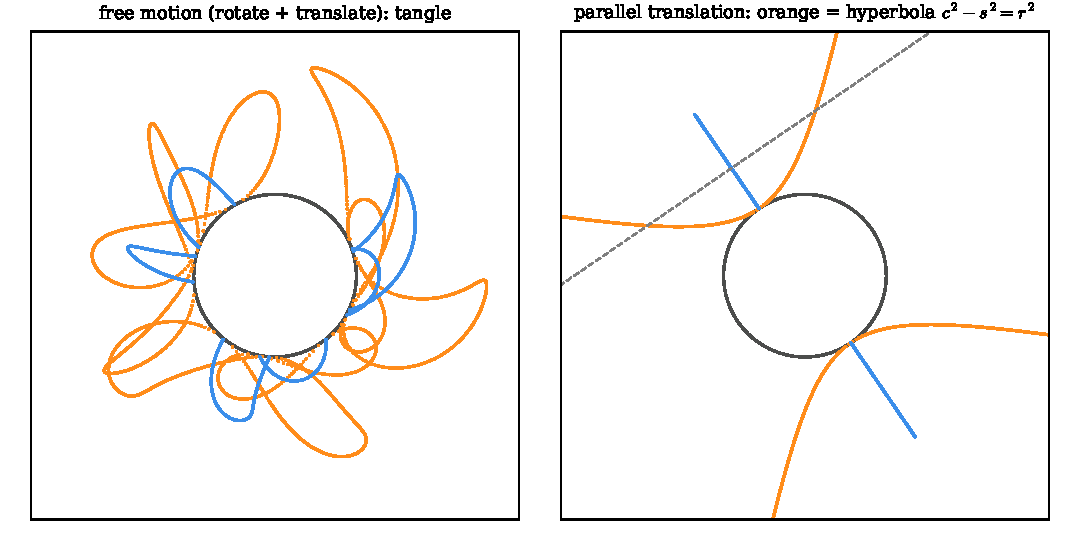
\includegraphics[width=\linewidth]{figs/fig2_quilez.pdf}
\caption{Quilez's construction ($r=1$). Blue: real part of the intersection; orange: real part $\pm$ imaginary part, drawn along the line. Left: free motion. Right: a fixed direction with only parallel translation. The orange trail is exactly the hyperbola $c^2-s^2=r^2$ in the line frame (numerical error $<10^{-14}$).}\label{fig:quilez}\end{figure}

\section{Setup: the line frame}
Let $F\in\R[x,y]$ have degree $k$ and put $X=\{F=0\}\subset\C^2$, with real points $X_\R=X\cap\R^2$. Fix a real unit direction $d$ and its normal $n=d^\perp$. Every $p\in\C^2$ can be written uniquely as
\[ p = c\,n + t\,d,\qquad (c,t)\in\C^2, \]
and we set $f(c,t)=F(cn+td)$, a real polynomial. The real lines parallel to $d$ are $L_c=\{n\cdot p=c\}$ with $c\in\R$; complexified, $L_c=\{(c,t):t\in\C\}$.

\begin{proposition}\label{prop:bezout}
For real $c$, $X\cap L_c$ is the root set of $t\mapsto f(c,t)$. This is a polynomial with \emph{real} coefficients, so its non-real roots come in conjugate pairs $a\pm ib$. Its leading coefficient is $F_k(d)$, the top-degree form of $F$ at $d$, which does not depend on $c$. So for every $c$ there are exactly $k$ roots counted with multiplicity, unless $d$ is an \emph{asymptotic direction} ($F_k(d)=0$), in which case some intersections lie at infinity for every $c$.
\end{proposition}
\noindent(Example: for $y=x^2$ with vertical lines, $f=t-c^2$ has degree $1$ in $t$.)

\begin{definition}
The \emph{line-real locus} of $X$ in direction $d$ is $X_d=X\cap(\R\times\C)$, viewed in $\R^3$ with coordinates $(\Re t,\,c,\,\Im t)$. Its part with $\Im t\neq0$ is the \emph{phantom locus} $\Phi_d(X)$, and $X_d=X_\R\cup\Phi_d(X)$.
\end{definition}

Away from points with $f_t=0$, the implicit function theorem gives $t=\tau(c)$ real-analytic in $c$, so $X_d$ is a real-analytic curve: \emph{one} real dimension inside the real surface $X$. This is the ``well-defined locus'' that parallel translation reveals. Free motion instead samples a 2-parameter family of lines, and its trail is a projection of an arbitrary path on the surface $X$.

\begin{figure}[t]\centering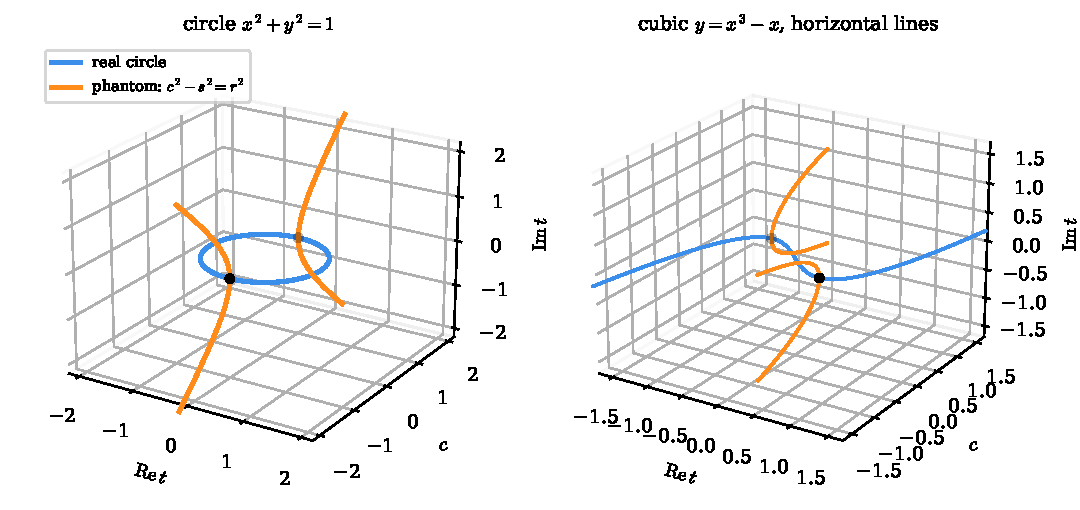
\includegraphics[width=\linewidth]{figs/fig1_locus3d.pdf}
\caption{Line-real loci $X_d$ in $(\Re t,c,\Im t)$. Blue: real curve. Orange: phantom. Black dots: tangency points. Left: the circle and its phantom hyperbola $c^2-s^2=1$ in the plane $\Re t=0$. Right: for $y=x^3-x$ the conjugate pairs have $\Re t\neq0$, so the phantom is not planar.}\label{fig:locus}\end{figure}

\section{Examples}
\textbf{Circle.} $x^2+y^2=r^2$ with any $d$ gives $f=c^2+t^2-r^2$. For $|c|>r$, $t=\pm i\sqrt{c^2-r^2}$, so with $s=\Im t$ the phantom is the hyperbola $c^2-s^2=r^2$ in the plane $\Re t=0$. In Quilez's construction with $o=hn+\tau d$, the orange dots are $hn\pm\sqrt{h^2-r^2}\,d$, which is the same hyperbola. His 2D picture is our 3D picture with the $\Im t$ axis folded onto $d$. Circle and hyperbola are two real slices of the single complex conic $X$, glued at the tangency points $(0,\pm r,0)$. Its asymptotes $c=\pm s$ correspond to $t=\pm ic$, i.e.\ the directions $n\pm i d$, which satisfy $(n\pm id)\cdot(n\pm id)=0$. These are the \emph{isotropic directions}, which point at the circle's two points at infinity (\S\ref{sec:iso}).

\textbf{Parabola.} $y=x^2$ with horizontal lines: $f=c-t^2$. For $c<0$, $t=\pm i\sqrt{-c}$, so the phantom is the inverted parabola $c=-s^2$.

\textbf{A generic cubic.} $y=x^3-x$ with horizontal lines: $f=t^3-t-c$. For $|c|>2/(3\sqrt3)$ there is one real root and a pair $a(c)\pm ib(c)$ with $a(c)\neq0$; e.g.\ at $c=0.6$, $t=-0.6106\pm0.3442i$. The phantom drifts off any plane (Fig.~\ref{fig:locus}, right). This shows that the ``imaginary-axis'' picture of the circle is special; see Proposition~\ref{prop:slice}.

\section{Tangency theorem}
\begin{theorem}\label{thm:tangency}
(a) The closure of $\Phi_d(X)$ meets the real plane $\{\Im t=0\}$ only at real points $(c_0,t_0)$ with $f=f_t=0$, i.e.\ zeros of the discriminant $\operatorname{Disc}_t f(c_0)$. Such a point is either a point where $L_{c_0}$ is tangent to $X_\R$ (a critical point of the height function $c=n\cdot p$ on $X_\R$) or a singular point of $X_\R$.\\
(b) Let the point be a smooth tangency of contact order $m\ge2$ ($f_c\neq0$, $\partial_t^jf=0$ for $j<m$, $\partial_t^mf\neq0$). Then exactly $m$ smooth branches of $X_d$ pass through it, with tangents in the $t$-plane at the equally spaced angles $\pi j/m$, $j=0,\dots,m-1$. The branch at angle $0$ is $X_\R$.\\
(c) For an ordinary tangency ($m=2$), write $c=c_0+\frac{\kappa}{2}(t-t_0)^2+\gamma(t-t_0)^3+\dots$ along $X$. Then $|\kappa|$ is the curvature of $X_\R$ at the point, and the phantom branch is
\[ c=c_0-\tfrac{\kappa}{2}\,(\Im t)^2+O(|\Im t|^3),\qquad \Re t-t_0=\tfrac{\gamma}{\kappa}\,(\Im t)^2+O(|\Im t|^3). \]
So the phantom leaves perpendicular to $X_\R$ and bends the opposite way, and its projection to the $(\Im t,c)$ plane has the same curvature $|\kappa|$. It stays in the plane $\Re t=t_0$ to second order exactly when $\gamma=0$.
\end{theorem}
\begin{proof}
(a) Suppose non-real roots $t_j$ of $f(c_j,\cdot)$ converge to a real $t_0$ as $c_j\to c_0$. Their conjugates $\bar t_j\neq t_j$ are also roots, and they converge to $t_0$ as well. By continuity of roots, $t_0$ is a root of $f(c_0,\cdot)$ of multiplicity at least $2$, so $f(c_0,t_0)=f_t(c_0,t_0)=0$. If $f_c\neq0$ there, $X$ is smooth with tangent line $f_c\,dc+f_t\,dt=0$, i.e.\ $dc=0$: the tangent is $L_{c_0}$, and the point is critical for $c$ on $X_\R$ (Lagrange). Otherwise $\nabla f=0$ and the point is singular.

(b) Since $f_c\neq0$, the implicit function theorem gives a holomorphic $g$ with $X=\{c=g(t)\}$ near the point. It has real Taylor coefficients and $g(t)=c_0+\alpha w^m(1+O(w))$ with $w=t-t_0$ and $\alpha\in\R^*$. The map $\zeta=w(1+O(w))^{1/m}$ is a conformal change of coordinates commuting with conjugation, and $g=c_0+\alpha\zeta^m$. So $X_d=\{g\in\R\}=\{\Im \zeta^m=0\}$, which is $m$ lines through $0$ at angles $\pi j/m$ in the $\zeta$-plane. Their conformal images are $m$ smooth curves with the same tangent angles.

(c) Write $w=u+iv$. Then $\Im g=\kappa uv+\gamma(3u^2v-v^3)+O(|w|^4)$. Dividing by $v$ on the non-real branch gives $\kappa u=\gamma v^2+O(v^3)$, and substituting into $\Re g$ gives $c=c_0-\frac\kappa2v^2+O(v^3)$. For real $t$, $c=g(t)$ is the graph of $X_\R$ over its tangent line, with $t$ the arclength coordinate, so its curvature at the critical point is $|g''(t_0)|=|\kappa|$.
\end{proof}

\noindent\emph{Numerical check.} For the cubic $x^2/4+y^2+x^2y/5=1$ with $d=(3/5,4/5)$, the tangency at $c_0=1.600953$ has $\kappa=-0.547942$ and $\gamma/\kappa=-0.304976$. Root tracking at $c_0+10^{-6}$ gives $(\Re t-t_0)/(\Im t)^2=-0.304975$ and $(c-c_0)/(-\kappa v^2/2)=0.999999$. For the inflection $y=x^3$ ($m=3$), the roots of $t^3=c$ lie on three lines at $0^\circ,\pm60^\circ$ (Fig.~\ref{fig:infl}). For $x^4+y^4=1$ along an axis ($m=4$), four lines lie at $0^\circ,45^\circ,90^\circ,135^\circ$ (Fig.~\ref{fig:quartic}).

\begin{figure}[t]\centering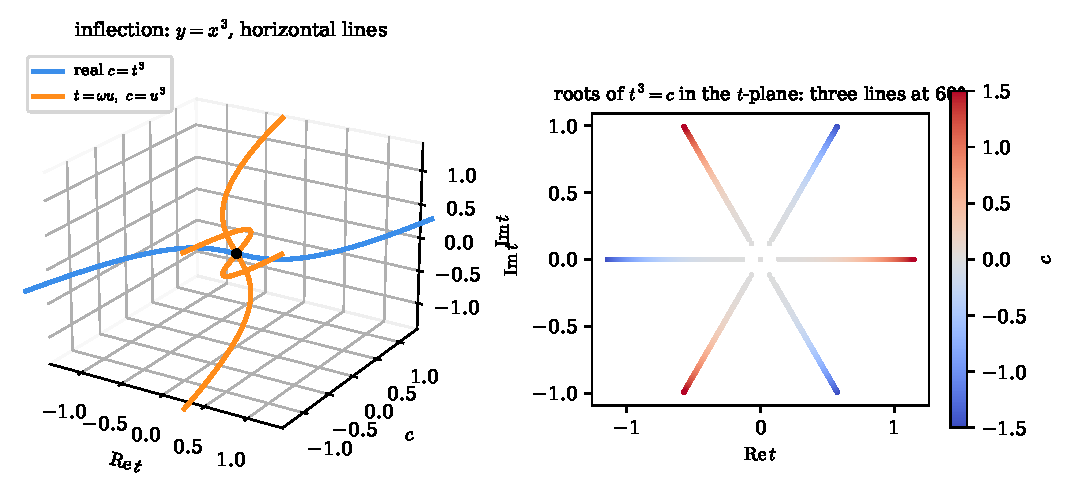
\includegraphics[width=\linewidth]{figs/fig4_inflection.pdf}
\caption{Inflection tangency $y=x^3$ (contact order 3). Left: the real cubic and the two conjugate branches $t=\omega u$, $c=u^3$, $\omega=e^{\pm2\pi i/3}$, all through the origin. Right: roots of $t^3=c$ coloured by $c$. Each complex branch crosses the origin along a straight line, so three lines meet at $60^\circ$.}\label{fig:infl}\end{figure}

\section{The operator and its group}
In the line frame define, for $\lambda\in\C^*$,
\[ R_\lambda:\C^2\to\C^2,\qquad (c,t)\mapsto(c,\lambda t),\qquad\text{i.e.}\quad R_\lambda=P_n+\lambda P_d . \]
Then $R_\lambda R_\mu=R_{\lambda\mu}$, $R_1=\mathrm{id}$ and $R_\lambda^{-1}=R_{1/\lambda}$, so $\lambda\mapsto R_\lambda$ is an injective homomorphism and $\{R_\lambda\}\cong\C^*$. The phantom operator is $R_i$. It has order $4$, and $R_i^2=R_{-1}$ is the mirror $t\mapsto-t$ across the $n$-axis. The group acts on curves by $R_\lambda\cdot X=R_\lambda(X)=\{f(c,t/\lambda)=0\}$, so $R_\lambda^{-1}(X)=\{f(c,\lambda t)=0\}$.

\begin{proposition}[Slices]\label{prop:slice}
For $|\lambda|=1$, the part of $X_d$ with $t\in\lambda\R$ is $R_\lambda\big(\text{real points of }R_\lambda^{-1}X\big)$. In particular
\[ \Phi_d(X)\cap\{\Re t=0\} \;=\; R_i\big(\{(c,s)\in\R^2: f(c,is)=0\}\big)\setminus\{s=0\}. \]
If $f$ is even or odd in $t$ (the curve is mirror-symmetric about the $n$-axis), $f(c,is)$ is a real or purely imaginary polynomial, so this slice is a real algebraic curve. If $f$ mixes parities, $f(c,is)=A+iB$ and the slice $A=B=0$ is generically finite: the phantom is \emph{not} the real part of $\{f(c,it)=0\}$.
\end{proposition}
\noindent So the slogan ``phantom $=$ real slice of $R_i^{-1}X$'' holds exactly for the circle and parabola. Even for symmetric curves it can describe only part of the phantom: for $x^4+y^4=1$ and $|c|>1$, the roots of $t^4=1-c^4$ lie on the diagonals $e^{\pm i\pi/4}\R$, which form the slice for $\lambda=e^{i\pi/4}$, namely $c^4-u^4=1$.

\textbf{Orbits.} The circle $c^2+t^2=r^2$ goes to $c^2+t^2/\lambda^2=r^2$. Real $\lambda$ gives all ellipses with the same $c$-semi-axis, and $\lambda=i$ gives the hyperbola. Circle, ellipses and hyperbola are one $\C^*$-orbit, isomorphic to $\C^*/\{\pm1\}$.

\begin{theorem}[Stabilizer]\label{thm:stab}
Let $f=\sum_k t^k f_k(c)$ be square-free and $K=\{k:f_k\neq0\}$. Put $\operatorname{Stab}(X)=\{\lambda\in\C^*:R_\lambda X=X\}$.
\begin{enumerate}
\item If $|K|=1$, $X$ is a union of lines $c=\mathrm{const}$ and possibly $t=0$, and $\operatorname{Stab}(X)=\C^*$.
\item If $|K|\ge2$, then $\operatorname{Stab}(X)=\mu_m$, the $m$-th roots of unity, where $m=\gcd\{k-k':k,k'\in K\}$.
\end{enumerate}
\end{theorem}
\begin{proof}
Square-free polynomials with the same zero set are proportional (Nullstellensatz). So $R_\lambda^{-1}X=X$ iff $f(c,\lambda t)=\mu f(c,t)$ for some $\mu\in\C^*$. Comparing coefficients of $t^k$ gives $\lambda^kf_k=\mu f_k$, i.e.\ $\lambda^k=\mu$ for all $k\in K$. If $|K|=1$ this holds for every $\lambda$ (take $\mu=\lambda^k$), and square-freeness forces $k\le1$. Otherwise it is equivalent to $\lambda^{k-k'}=1$ for all $k,k'\in K$. The differences generate the subgroup $m\Z\subset\Z$, so the condition is $\lambda^m=1$, which forces $|\lambda|=1$. The stabilizer is closed under inverses, so $R_\lambda X=X$ gives the same set.
\end{proof}
\begin{corollary}[Self-phantom curves]
$R_i X=X$ iff $4\mid m$, i.e.\ all exponents of $t$ in $f$ are congruent mod $4$. Then the real points of $R_i^{-1}X$ coincide with $X_\R$: the imaginary slice of the phantom is an exact copy of the real curve, rotated into the $\Im t$ direction. Likewise $R_{-1}X=X$ iff $m$ is even (mirror symmetry).
\end{corollary}
\noindent\emph{Examples} (all confirmed by brute force over $48$-th roots of unity): $K=\{0,2\}$ (circle) gives $m=2$; $\{0,2,4\}$ gives $2$; $\{0,4\}$ gives $4$; $\{1,5\}$ gives $4$; $\{0,3\}$ gives $3$; $\{2,8\}$ gives $6$; $\{1,4,7\}$ gives $3$; $\{0,1\}$ gives $1$.

\begin{figure}[t]\centering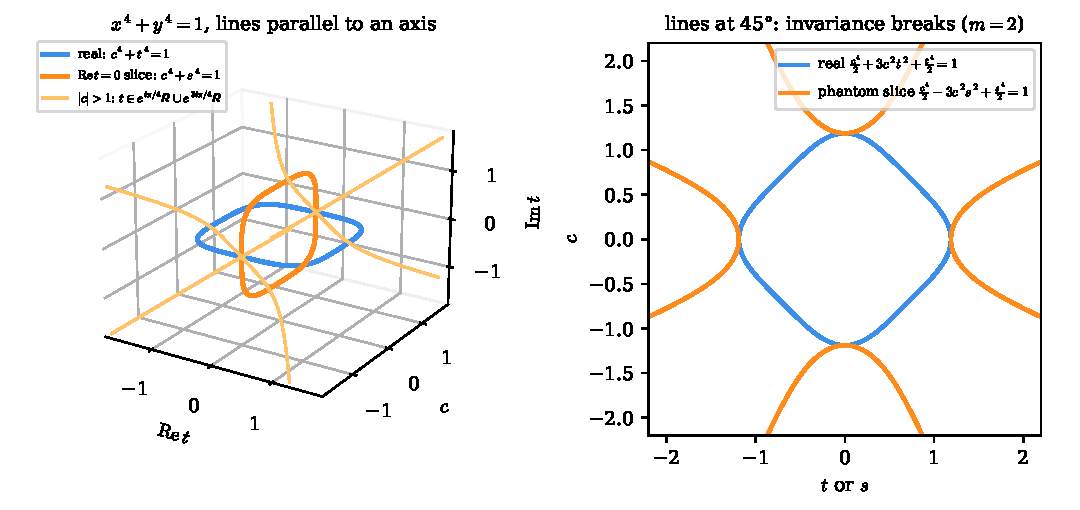
\includegraphics[width=\linewidth]{figs/fig3_quartic.pdf}
\caption{$x^4+y^4=1$. Left: along an axis, $f=c^4+t^4-1$, $K=\{0,4\}$, $m=4$. The $\Re t=0$ slice (orange) is an exact copy of the real curve (blue), and for $|c|>1$ the remaining phantom branches lie in the diagonal planes. Right: at $45^\circ$, $f=\tfrac12c^4+3c^2t^2+\tfrac12t^4-1$, $K=\{0,2,4\}$, $m=2$. The imaginary slice $\tfrac12c^4-3c^2s^2+\tfrac12s^4=1$ is a different, unbounded curve that touches the real one at the tangencies $c=\pm2^{1/4}$.}\label{fig:quartic}\end{figure}

\begin{remark}
$K$ and $m$ depend on the frame: on $d$, and on the choice of the axis $t=0$. Translating $t\mapsto t+a$ changes $K$. For example, a circle centred off the axis has $K=\{0,1,2\}$ and $m=1$. ``Self-phantom'' is a property of the curve together with a line direction and an axis, not of the curve alone. The circle is special because $m=2$ for every $d$ through its centre, but no real direction gives $m=4$ for it.
\end{remark}

\section{Inversive geometry: keeping the operator inside the space of circles}\label{sec:inv}
The operator $R_i$ turns a circle into a hyperbola, so it leaves the family of circles. Inversive (Möbius) geometry treats circles and lines as one kind of object, which suggests a better question: is there a version of the ``hidden $\leftrightarrow$ visible'' swap that stays inside the space of circles?

\subsection{The space of circles}
A generalized circle is $a(x^2+y^2)+bx+cy+d=0$, up to scale, i.e.\ a point $[a:b:c:d]\in\mathbb{P}^3$. Lines are the case $a=0$, and $\infty:=[0:0:0:1]$ is the point at infinity. Put
\[ Q(C)=b^2+c^2-4ad,\qquad \langle C_1,C_2\rangle=b_1b_2+c_1c_2-2(a_1d_2+a_2d_1). \]
Since $Q=b^2+c^2+(a-d)^2-(a+d)^2$, the form has signature $(3,1)$. For $a\neq0$ the centre is $(-b/2a,-c/2a)$ and $Q=4a^2r^2$. So $Q>0$ is a real circle (every real line has $Q=b^2+c^2>0$), $Q=0$ a point circle, and $Q<0$ an imaginary circle such as $x^2+y^2+1=0$ ($Q=-4$). A point $p$ is the point circle $P(p)=[1:-2x:-2y:|p|^2]$, and
\[ \langle P(p),C\rangle=-2\,C(p), \]
so \emph{incidence is orthogonality}: $p\in C\iff P(p)\perp C$. The points of the inversive plane $\R^2\cup\{\infty\}\cong S^2$ form the null quadric $\{Q=0\}$. For two real circles with radii $r_1,r_2$ and centre distance $\delta$, $\langle C_1,C_2\rangle/\sqrt{Q_1Q_2}=(r_1^2+r_2^2-\delta^2)/(2r_1r_2)=\cos\theta$, where $\theta$ is the intersection angle. For a circle and a line, the same ratio is $\pm\delta/r$, with $\delta$ the distance from the centre to the line. Hence:

\begin{proposition}\label{prop:inv}
For real circles or lines $C_1,C_2$, let $I=\langle C_1,C_2\rangle^2/(Q_1Q_2)$. Then $I<1$ means two real intersection points (at angle $\theta$, $I=\cos^2\theta$), $I=1$ means tangency, and $I>1$ means a conjugate pair of intersection points. For $C_0:x^2+y^2=r^2$ and $L_c:y=c$ (with $d=(1,0)$, $n=(0,1)$), $I=c^2/r^2$.
\end{proposition}
\noindent(Checked on 3000 random circle pairs and 3000 random circle–line pairs: no mismatches, and $|I-\cos^2\theta|<2\cdot10^{-14}$.)

\subsection{The Möbius group}
Inversion in a real circle $C$ acts on $\R^{3,1}$ as the reflection $X\mapsto X-2\frac{\langle X,C\rangle}{Q(C)}C$ (checked numerically to $10^{-12}$). Inversions generate the Möbius group, so it acts \emph{linearly} on circles preserving $Q$: $\mathrm{M\ddot ob}\cong PO(3,1)$, whose orientation-preserving part is $PSO^+(3,1)\cong PSL(2,\C)$. Complexifying gives $PO(4,\C)$, acting on complex circles $\mathbb{P}^3(\C)$ and on the complex null quadric $\{Q=0\}\cong\mathbb{P}^1\times\mathbb{P}^1$, with coordinates $z=x+iy$, $w=x-iy$ on the finite part $\C^2$. The identity component is $PSO(4,\C)\cong PSL(2,\C)\times PSL(2,\C)$, acting by $(z,w)\mapsto(g z,h w)$. The real Möbius plane is the fixed set of the real structure $\sigma_0:(x,y)\mapsto(\bar x,\bar y)$, i.e.\ $w=\bar z$. The two rulings $z=\mathrm{const}$ and $w=\mathrm{const}$ of the quadric are the isotropic lines of \S\ref{sec:iso}.

\subsection{Point pairs as 2-planes}
A pair of points $\{P_1,P_2\}$ (a $0$-sphere) is a 2-plane $U=\mathrm{span}(P_1,P_2)\subset\R^{3,1}$, a line in $\mathbb{P}^3$ meeting the quadric in $P_1,P_2$. Two circles $C_1,C_2$ meet in the null points of $U=V^\perp$, where $V=\mathrm{span}(C_1,C_2)$ is the \emph{pencil} (coaxal system) they span. Because the total signature is $(3,1)$, a real 2-plane is of exactly one of three types:
\begin{center}\begin{tabular}{llll}
signature of $U$ & null points of $U$ & $V=U^\perp$ & $\det\mathrm{Gram}(C_1,C_2)=Q_1Q_2-\langle C_1,C_2\rangle^2$\\\hline
$(1,1)$ & real pair & $(2,0)$: elliptic pencil & $>0$ \ ($I<1$)\\
degenerate & double point & parabolic pencil & $=0$\\
$(2,0)$ & conjugate pair $P,\bar P$ & $(1,1)$: hyperbolic pencil & $<0$ \ ($I>1$)
\end{tabular}\end{center}
The signature $(0,2)$ cannot occur. For a conjugate pair, $u=P+\bar P$ and $v=i(P-\bar P)$ span a real plane with $Q|_U=2\langle P,\bar P\rangle(u^2+v^2)$, which must be positive definite. The null points of $V$ itself are the \emph{limiting points} of the pencil. They are real exactly when the intersection pair is imaginary, and vice versa.

\begin{proposition}[Polarity swaps real and imaginary pairs]\label{prop:polar}
The map $U\mapsto U^\perp$ on point pairs is a Möbius-equivariant involution exchanging real pairs and conjugate pairs. For $C_0$ and $L_c$ it sends the intersection pair $C_0\cap L_c=\{(\pm\sqrt{r^2-c^2},\,c)\}$ to the limiting points
\[ \{(0,\;c\pm\sqrt{c^2-r^2})\}, \]
which are mutually inverse in $C_0$ (the product of their $y$-coordinates is $r^2$). For $|c|>r$, with $s=\sqrt{c^2-r^2}$, the hidden pair $(\pm is,c)$ becomes the real pair $(0,c\pm s)$ on the normal through the foot $(0,c)$. Quilez's orange dots $(\pm s,c)$ are the same real pair rotated by $90^\circ$ about the foot.
\end{proposition}
\begin{proof}
$U\mapsto U^\perp$ commutes with every element of $PO(3,1)$, and the table shows it swaps the $(1,1)$ and $(2,0)$ types. With $C_0=[1:0:0:-r^2]$ and $L_c=[0:0:1:-c]$, $Q(\lambda C_0+\mu L_c)=4r^2\lambda^2+4c\lambda\mu+\mu^2$ vanishes at $\mu/\lambda=-2c\pm2\sqrt{c^2-r^2}$. The circle $x^2+y^2+\mu y-r^2-\mu c=0$ then has radius $0$ and centre $(0,-\mu/2)=(0,c\mp\sqrt{c^2-r^2})$.
\end{proof}
\noindent(Numerically, for $r=1$: at $c=1.7$ the null points of $U$ are $(\pm1.37477i,1.7)$ and those of $V$ are $(0,3.07477),(0,0.32523)$. At $c=0.6$ they are $(\pm0.8,0.6)$ and $(0,0.6\pm0.8i)$.)

\begin{figure}[t]\centering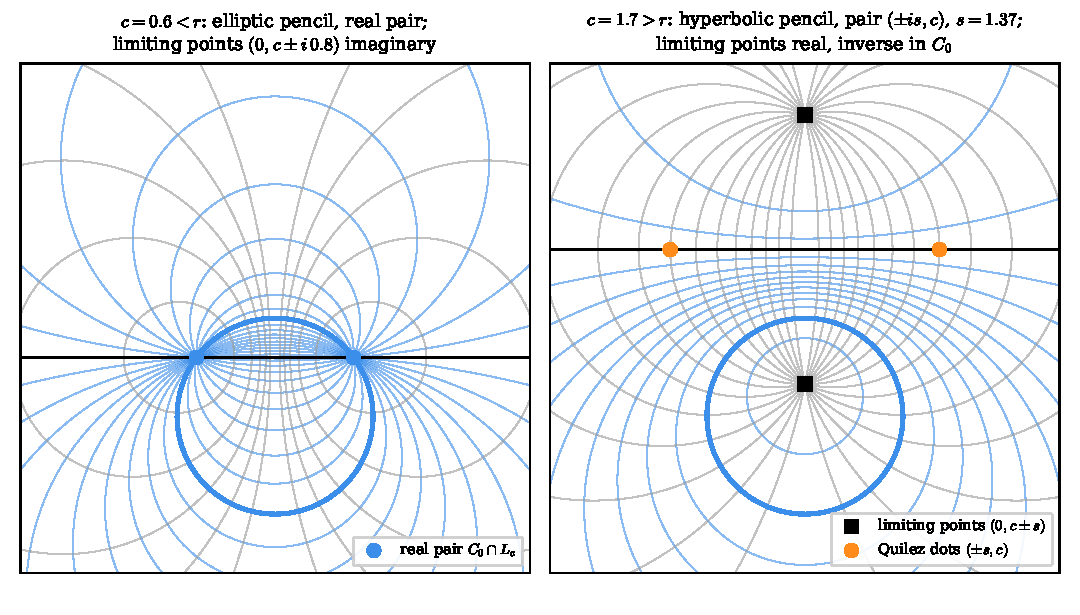
\includegraphics[width=\linewidth]{figs/fig5_pencil.pdf}
\caption{The pencil $V_c=\mathrm{span}(C_0,L_c)$ (thin blue) and its orthogonal pencil $V_c^\perp$ (grey), for $r=1$. Left, $c=0.6$: elliptic pencil through the real pair $C_0\cap L_c$, with imaginary limiting points. Right, $c=1.7$: the pair is $(\pm is,c)$; the pencil is hyperbolic with real limiting points $(0,c\pm s)$ (squares), through which every grey circle passes. Quilez's dots $(\pm s,c)$ (orange) are the limiting points rotated by $90^\circ$ about the foot $(0,c)$.}\label{fig:pencil}\end{figure}

\subsection{Why \texorpdfstring{$R_i$}{R\_i} is not internal, and what replaces it}
Write $M=R_{-1}:(x,y)\mapsto(-x,y)$ for the mirror in the $n$-axis, which is a real Möbius map.

\begin{theorem}\label{thm:inv}
Let $C_0:x^2+y^2=r^2$ and the parallel pencil $\mathcal{P}=\{L_c:y=c\}$.
\begin{enumerate}
\item $R_i$ is not induced by any element of $PO(4,\C)$. It sends the circular points $(1:\pm i:0)$ to the real points $(1:\pm1:0)$, so it sends circles (conics through the circular points) to non-circles; $C_0$ goes to the hyperbola $y^2-x^2=r^2$.
\item The subgroup of $PO(4,\C)$ preserving $C_0$ and $\mathcal{P}$ is the Klein four-group $\{\mathrm{id},\,-\mathrm{id},\,M,\,(x,y)\mapsto(x,-y)\}$. It consists of real maps and contains $R_i^2=M$, but not $R_i$. So no element of the complexified circle group fixing the configuration exchanges real and imaginary point pairs.
\item The exchange is a \emph{change of real structure}. Let $\sigma_1=\sigma_0\circ M:(x,y)\mapsto(-\bar x,\bar y)$. It is an anti-holomorphic involution that preserves the circle family and fixes $C_0$ and every $L_c$, and $\sigma_1=R_i\sigma_0R_i^{-1}$. On each pair $C_0\cap L_c$, $\sigma_0$ fixes both points when $|c|<r$ and swaps them when $|c|>r$, while $\sigma_1$ does the opposite. The $\sigma_1$-real points of $C_0$ are $\{(is,c):c^2-s^2=r^2\}$, the phantom hyperbola.
\item The $\sigma_1$-real circles are $[a:i\beta:c:d]$ with $a,\beta,c,d$ real, on which $Q=-\beta^2+c^2-4ad$ has signature $(2,2)$. So $\sigma_1$ is the real form $PO(2,2)$ of $PO(4,\C)$: the conformal geometry of the \emph{Lorentzian} plane $\{(is,c)\}$ with metric $dc^2-ds^2$, whose ``circles'' are hyperbolas. In that geometry, the phantom of the circle is the Lorentzian circle of the same radius.
\end{enumerate}
\end{theorem}
\begin{proof}
(1) $R_i$ multiplies the top-degree form $x^2+y^2$ into $y^2-x^2$, which does not vanish at $(1:\pm i)$. Equivalently, the induced map on point vectors $[1:-2x:-2y:x^2+y^2]\mapsto[1:-2ix:-2y:y^2-x^2]$ is not linear: the best linear fit on 12 random points leaves residual $2.04$.
(2) Every pencil member passes through $\infty$, and $\infty$ is the only base point of $\mathcal{P}$ (the null points of $\mathcal{P}^\perp$ reduce to $[0:0:0:1]$). So the stabilizer fixes $\infty$ and consists of complex similarities $(z,w)\mapsto(\alpha z+a,\beta w+b)$, or the same composed with $z\leftrightarrow w$. Preserving $zw=r^2$ forces $a=b=0$ and $\alpha\beta=1$. Mapping the lines $z-w=2ic$ to lines of the same form forces $\alpha=\beta$. Hence $\alpha=\pm1$ (solved symbolically).
(3) For $\sigma_1=R_i\sigma_0R_i^{-1}$: $(x,y)\mapsto(-ix,y)\mapsto(i\bar x,\bar y)\mapsto(-\bar x,\bar y)$. $\sigma_1$ preserves circles because $\sigma_0$ and $M$ do. On $C_0\cap L_c=\{(\pm\xi,c)\}$, $\sigma_0$ fixes each point iff $\xi\in\R$, and $\sigma_1(\xi,c)=(-\bar\xi,c)$ fixes each point iff $\xi\in i\R$.
(4) Points fixed by $\sigma_1$ are $(is,c)$ with $s,c$ real, and $P(is,c)=[1:-2is:-2c:c^2-s^2]$ has the stated form.
\end{proof}

\noindent\textbf{Summary.} Inside the space of circles there are two honest replacements for $t\mapsto it$, and neither is a group element fixing the configuration.
(a) The \emph{polarity} $U\mapsto U^\perp$ is a real, Möbius-equivariant operation on point pairs. It sends the hidden pair of $C_0$ and $L_c$ to the real limiting points of the pencil they span.
(b) Swapping which points count as real is a change of real form, $PO(3,1)\to PO(2,2)$, implemented by $\sigma_1=\sigma_0M$. The two real forms are not conjugate in $PO(4,\C)$, because a conjugating element would carry a real 4-space of signature $(3,1)$ to one of signature $(2,2)$ while scaling $Q$. In this language, $R_i$ is a square root of the Möbius mirror $M$ that lives outside the Möbius group and intertwines the two real structures. The circle and its phantom are one complex circle, seen through the Euclidean and the Lorentzian real structure.

\section{Isotropic directions and open questions}\label{sec:iso}
All of the above uses a real unit $d$. Allowing $d\in\C^2$, the frame $p=cn+td$ needs $d\cdot d\neq0$. The degenerate directions are the isotropic ones, $d=(1,\pm i)$ with $d\cdot d=0$. For these, $n=d^\perp$ is parallel to $d$, the splitting $\C^2=\C n\oplus\C d$ collapses, and $R_\lambda=P_n+\lambda P_d$ (with $P_d=dd^{\mathsf T}/(d\cdot d)$) is undefined. They are the eigenlines of the complex rotations $SO(2,\C)$, and $x^2+y^2=(x+iy)(x-iy)$ factors along them. An isotropic line meets the circle in only one finite point, since $(x_0+t)^2+(y_0+it)^2-r^2=x_0^2+y_0^2-r^2+2t(x_0+iy_0)$ is linear in $t$. The other point is at a circular point at infinity $(1:\pm i:0)$. These are also the directions of the phantom hyperbola's asymptotes. Open directions:
\begin{enumerate}
\item \emph{The full group.} Which group is generated by all $R^{(d)}_\lambda$ as $d$ ranges over the non-isotropic directions? It contains all reflections ($\lambda=-1$), hence $O(2)$, and axis-parallel scalings. Which curves have a non-trivial stabilizer under it? (Within the Möbius group, \S\ref{sec:inv} shows the stabilizer of a circle and a parallel pencil is only a Klein four-group.)
\item \emph{The isotropic limit.} Describe $X_d$ as $d\to(1,\pm i)$ and relate the phantom's asymptotic behaviour to the points of $X$ at infinity (the circular points for circles).
\item \emph{Global topology.} The union of the $X_d$ over all real $d$ sweeps the real surface $X$. How do the tangency points of Theorem~\ref{thm:tangency} (critical points of the height function) organize it, in the spirit of Morse theory?
\item \emph{Mixed parity.} For curves without mirror symmetry the phantom is not a linear image of a real curve (Prop.~\ref{prop:slice}). Is there a natural non-linear operator, e.g.\ one centred at $a(c)=\Re t$, that restores the slice picture?
\end{enumerate}

\paragraph{Reproducibility.} \texttt{verify.py} checks every numerical statement (log in \texttt{verify\_log.txt}), \texttt{verify\_inversive.py} checks \S\ref{sec:inv} (log in \texttt{verify\_inversive\_log.txt}), and \texttt{figs.py}, \texttt{fig\_pencil.py} produce the figures.
\end{document}
